%\chapter{開発プロセス}
\section{第4サイクル}
第4サイクルは外部講師のリモートレビューが終わった日から12月11日のプロジェクト最終報告会までとした。本サイクルでは、第3サイクルでは進めていた実装をさらに進めること、そしてカルタに代わる何か手間のかからない「もの」を提案することを課題として活動を行った。
\par カルタ以外で手間がかからないものは何かを議論し合った結果、リーフレット\footnote{一枚刷りの印刷物、折りたたみ式の小型の印刷物}という案が生まれた。カルタのような数の手間をかけず、さらに一枚の紙で作成できて低コストに抑えられるため、この案を採用した。しかし、必ずしもユーザがリーフレットを印刷するとも限らないため、アプリ内でも振り返られるようにアルバム機能を作ることを決定した。本サイクルで実装した機能は大きく分けて、観光する機能、振り返る機能、そして印刷する機能の3つを実装した。11月14日にアカデミックリンクがあったため、一旦そこをマイルストーンとして開発し、多くの企業の方や一般の方からレビューを受けた。そのレビューを受けて最終報告会までさらに開発を続けた。具体的に実装した機能・画面は次章で詳説する。前回のサイクルと本サイクルでの主な変化を表5.3に、リーフレットの完成サンプルを図5.7に示す。
\par 本サイクルでは長く続けてきた要件定義が充分に固まったため、比較的実装に集中できて完成度の高いアプリを開発で来た。最終報告会での評価も高かったため、今後はプロジェクトが終わっても開発を続けてリリースをすることになった。そのために、今後は木古内の関係者の方々にキーコ紀行を実際に提案しに行き現地の人のレビューを貰ってさらに質の高いアプリにすること、現在生じているバグを取り除くこと、そしてどのように運営をやっていくかを決定することが当面の課題となるだろう。

\begin{table}[htb]
\centering
\addtocounter{table}{+0}
\caption{第3サイクルから第4サイクルへの変化}
  \begin{tabular}{|l|l|} \hline
    改正前&改正後  \\ \hline 
    カルタを作る機能 & \parbox{20zw}{リーフレットを自動生成する機能} \\  \hline
    カルタから思い出を振り返る &\parbox{20zw}{アルバム機能または、リーフレットを用いて思い出を振り返る}\\ \hline
  \end{tabular} 
\end{table}

\begin{figure}[htbp]
  \begin{center}
    \begin{tabular}{c}
      % 1
      \begin{minipage}{0.33\hsize}
        \begin{center}
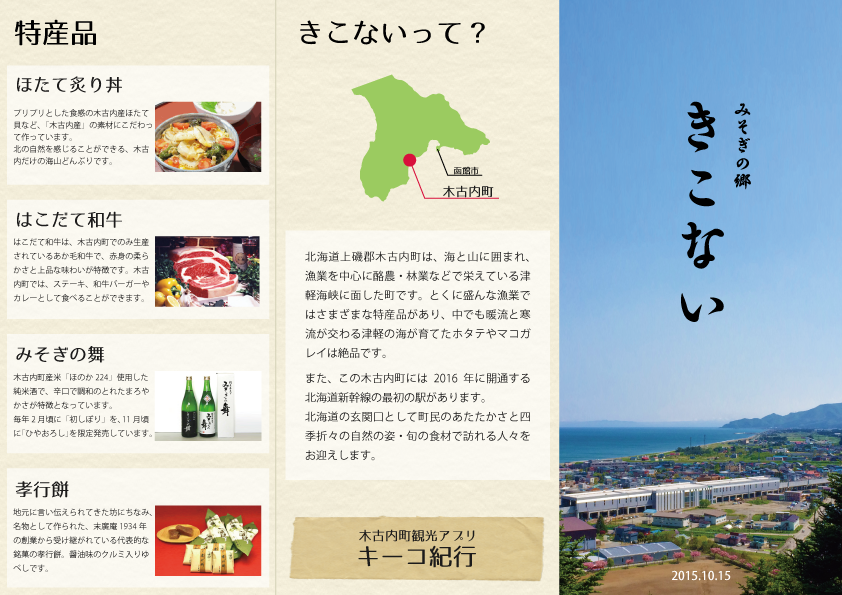
\includegraphics[width=6cm, bb=0 0 640 1104]{leaflet_front.png}
	\hspace{1cm} (a)リーフレット表側
        \end{center}
      \end{minipage}

      % 2
      \begin{minipage}{0.33\hsize}
        \begin{center}
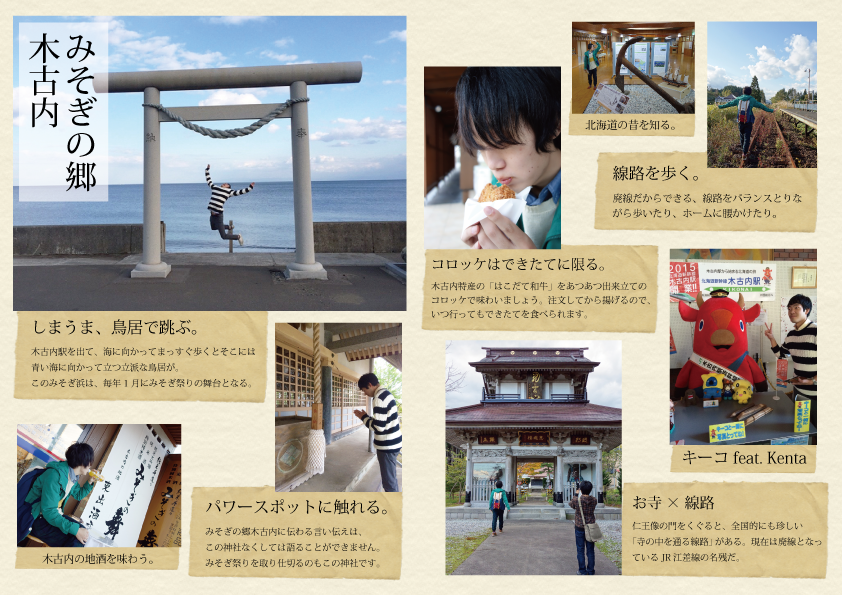
\includegraphics[width=6cm, bb=0 0 642 1094]{leaflet_back.png}
      	\hspace{1cm} (b)リーフレット裏側
	\end{center}
      \end{minipage}

    \end{tabular}
  \end{center}
\addtocounter{figure}{+0}
 \caption{リーフレット完成サンプル}
\end{figure}

\begin{description}
\item[アカデミックリンクでのレビュー内容]\mbox{}
 \begin{itemize}
 \item 継続的に使ってもらう仕組みが足りていない。
 \item フォントが統一されていない。
 \item リーフレットの写真をもう少しまとめてほしい。
 \item デザイン面をもう少し改善してほしい。ボタンのアイコンや色の配色等。
 \end{itemize}
\item[最終報告会でのレビュー内容]\mbox{}
 \begin{itemize}
 \item 利便性とカスタマイズできる点が面白い。
 \item アプリをどうやって広めていくのかがあまりわからなかった。
 \item 自分だけのリーフレットを作れるのは面白い。
 \item 拡張の可能性を感じる。
 \item もっと木古内らしさを出してほしい。
 \item リーフレット作ってもゴミになってしまうのでは。
 \item 操作説明が欲しい。
 \item 検索機能が欲しい。
 \item データではなくものにできるのは良い。
 \item UIデザインが分かりやすい。
 \item 観光情報が分かりやすくまとまっている。
 \item 写真が無駄にならなくて済む。
 \end{itemize}
\end{description}

\bunseki{山川拓也}